\documentclass[11pt, a4paper]{article}

\usepackage[T1]{fontenc}
\usepackage[utf8]{inputenc}
\usepackage[english]{babel}
\usepackage{lmodern}
\usepackage{microtype}
\usepackage[top=2.0cm, bottom=2.2cm, left=1.8cm, right=1.8cm]{geometry}
\usepackage{booktabs}
\usepackage{float}
\usepackage[table]{xcolor}
\usepackage{hyperref}
\hypersetup{colorlinks=true, linkcolor=darkblue, citecolor=darkblue, urlcolor=darkblue}
\usepackage{graphicx}
\usepackage{titlesec}
\usepackage{fancyhdr}
\usepackage{parskip}
\usepackage{amsmath}
\usepackage{amssymb}
\usepackage{tikz}
\usetikzlibrary{arrows.meta, positioning, shapes.geometric}
\usepackage{caption}
\captionsetup{font=small, labelfont=bf}

\definecolor{darkblue}{RGB}{26, 60, 120}

\titleformat{\section}
  {\large\bfseries\color{darkblue}}
  {\thesection.}{0.6em}{}[\vspace{-4pt}\rule{\linewidth}{0.4pt}]

\titleformat{\subsection}
  {\normalsize\bfseries\color{darkblue}}
  {\thesubsection}{0.6em}{}

\pagestyle{fancy}
\fancyhf{}
\fancyhead[L]{\small\textcolor{gray}{TER -- Monthly Report}}
\fancyhead[R]{\small\textcolor{gray}{M1 MLDM -- UJM Saint-Etienne}}
\fancyfoot[C]{\small\thepage}
\renewcommand{\headrulewidth}{0.3pt}

\setcounter{secnumdepth}{2}

\begin{document}

\begin{titlepage}
    \centering
    \vspace*{1.5cm}
    {\large\color{darkblue}\textbf{Universite Jean Monnet Saint-Etienne}}\\[0.3em]
    {\normalsize TER -- S2 2025/2026}

    \vspace{1.5cm}
    {\color{darkblue}\rule{\linewidth}{1.5pt}}
    \vspace{0.6cm}

    {\LARGE\bfseries\color{darkblue} Design and Evaluation of a Legal AI Assistant:\\
    A Comparative Study of RAG and Fine-Tuning}

    \vspace{0.4cm}
    {\large Monthly Progress Report -- June/July 2026}
    \vspace{0.6cm}

    {\color{darkblue}\rule{\linewidth}{1.5pt}}
    \vspace{1cm}

    
\includegraphics[width=0.4\linewidth]{latex_assets/UJM-LOGO-NOIR.png}
    \vspace{1.5cm}

    {\large\bfseries Author}\\[0.8em]
    \begin{tabular}{c}
        {\large Chaabane Ouammou} \\[0.3em]
        \small M1 MLDM\\
    \end{tabular}

    \vspace{0.6cm}
    \begin{tabular}{c}
        {\normalsize Co-author: Bartosz Konior} \\[0.2em]
        \small M1 DSC\\
    \end{tabular}

    \vspace{1cm}
    \begin{tabular}{rl}
        \textbf{Advisor:} & Marc Sebban \\[0.3em]
    \end{tabular}
\end{titlepage}

\pagecolor{white}
\color{black}
\setcounter{page}{1}
\twocolumn

\section{Scope of This Phase}

The previous phase of this project established a first working pipeline for both adaptation strategies and produced a first, single-run comparison between them. Since then the experimental surface has grown substantially, in scale, in the number of configurations examined and in the number of angles from which the same underlying question is approached. This report describes that extension, the reasoning behind each new experiment and what each one taught us that the previous, smaller comparison could not show. Rather than repeating the description of the dataset and the two adaptation strategies already given in the previous report, this document picks up the thread where it was left and follows the evolution of our reasoning through the results themselves.

Two adaptation strategies remain compared throughout. Retrieval-augmented generation retrieves the statutory articles most relevant to a question and places them in the model prompt before generation. Fine-tuning with QLoRA instead adjusts a small number of additional weights inside the model itself, so that the adapted behaviour is baked into the network rather than supplied as context at inference time. A third possibility, combining both, was added this phase specifically because the previous report could not say whether the two techniques address the same weakness or two different ones. That question turned out to be central and runs through most of the sections below.

\section{Retrieval Evaluated More Carefully}
\label{sec:retrieval}

The retrieval step decides which statutory articles the generator ever sees. If the right article is never retrieved, no amount of generation quality can recover the correct answer, so it made sense to examine this component in isolation and with more care than a single embedding model allowed.

Retrieval quality is measured with three complementary metrics rather than one, because each one answers a slightly different practical question. Recall at rank $k$ asks how often the correct article appears anywhere among the top $k$ results returned for a question, which matters directly for our RAG pipeline since only the top $k$ articles are ever shown to the generator. Writing $g_q$ for the gold article of question $q$ and $R_q^{(k)}$ for the set of the $k$ highest scoring articles retrieved for $q$, recall at $k$ over a set of questions $Q$ is

\begin{equation}
\text{Recall@}k = \frac{1}{|Q|} \sum_{q \in Q} \mathbb{1}\!\left[g_q \in R_q^{(k)}\right].
\end{equation}

Mean reciprocal rank looks instead at how far down the ranked list the correct article sits, which recall alone cannot express since it treats every article inside the top $k$ identically whether it is ranked first or last. With $\text{rank}_q$ the position of the gold article in the ranked list (or infinity if absent from the top 10),

\begin{equation}
\text{MRR@}10 = \frac{1}{|Q|} \sum_{q \in Q} \frac{1}{\text{rank}_q}.
\end{equation}

Normalized discounted cumulative gain is included as a third view because it weights a correct result found at rank one more heavily than one found at rank ten, in a smoother way than recall or MRR, which is useful when several gold articles can be relevant to the same question rather than a single one.

Retrieval itself relies on embedding every article and every question into the same vector space and comparing them by cosine similarity, $\text{sim}(q,d) = \frac{q \cdot d}{\lVert q \rVert \, \lVert d \rVert}$, so that semantically close texts end up numerically close even when they share few exact words, which is the property a purely lexical method such as BM25 does not have. The general purpose sentence embedding model used previously was replaced this phase by \texttt{intfloat/multilingual-e5-large}, a larger multilingual model that expects a distinct prefix for passages and for queries, and a lexical BM25 baseline and a hybrid combination of the two (reciprocal rank fusion of the BM25 and dense rankings) were added for comparison.

\begin{figure*}[t]
\centering
\resizebox{\textwidth}{!}{%
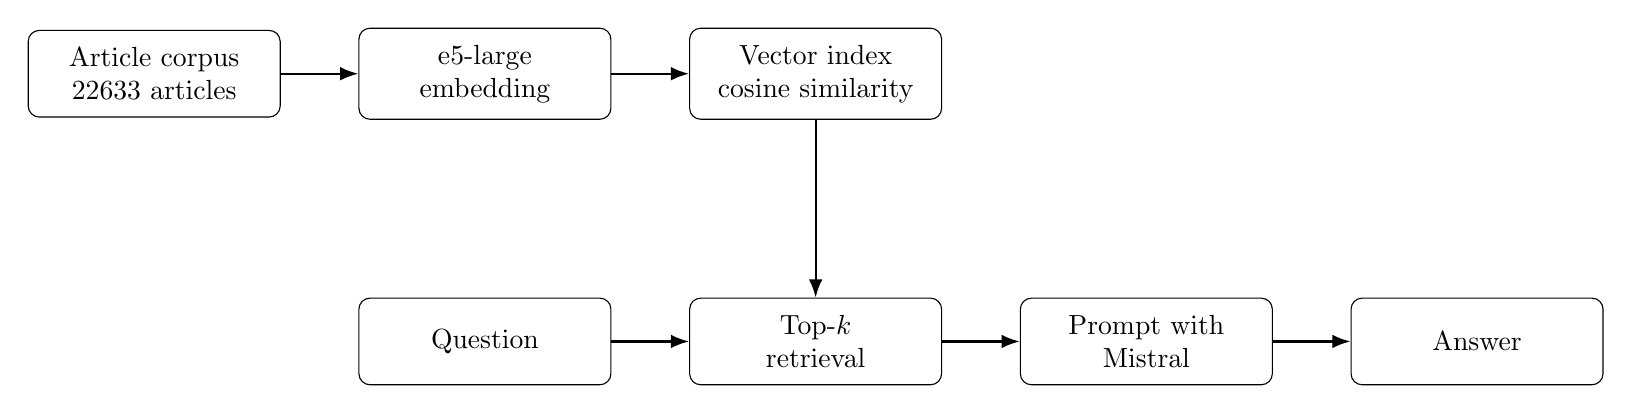
\begin{tikzpicture}[
  box/.style={draw, rounded corners, minimum height=1.1cm, minimum width=3.2cm, align=center, font=\normalsize, inner sep=6pt},
  arr/.style={-{Latex}, thick}
]
\node[box] (corpus) at (0,3.4) {Article corpus\\22633 articles};
\node[box] (embed)  at (4.2,3.4) {e5-large\\embedding};
\node[box] (index)  at (8.4,3.4) {Vector index\\cosine similarity};
\node[box] (question) at (4.2,0) {Question};
\node[box] (retrieve) at (8.4,0) {Top-$k$\\retrieval};
\node[box] (prompt)   at (12.6,0) {Prompt with\\Mistral};
\node[box] (answer)   at (16.8,0) {Answer};
\draw[arr] (corpus) -- (embed);
\draw[arr] (embed) -- (index);
\draw[arr] (index) -- (retrieve);
\draw[arr] (question) -- (retrieve);
\draw[arr] (retrieve) -- (prompt);
\draw[arr] (prompt) -- (answer);
\end{tikzpicture}}
\caption{Retrieval-augmented generation pipeline. The corpus is embedded once, offline, and indexed for cosine similarity. At inference time a question is embedded the same way, compared against the index, and the retrieved articles are placed alongside the question in the prompt given to Mistral.}
\label{fig:ragdiagram}
\end{figure*}

\begin{table*}[t]
\centering
\begin{tabular}{lccccc}
\toprule
\textbf{Method} & \textbf{R@1} & \textbf{R@5} & \textbf{R@10} & \textbf{MRR@10} & \textbf{nDCG@10} \\
\midrule
BM25 & 0.063 & 0.184 & 0.224 & 0.215 & 0.176 \\
mpnet (previous) & 0.021 & 0.074 & 0.097 & 0.105 & 0.076 \\
e5-large & 0.083 & 0.211 & 0.296 & 0.288 & 0.230 \\
Hybrid BM25+e5 & 0.106 & 0.250 & 0.322 & 0.312 & 0.258 \\
\bottomrule
\end{tabular}
\caption{Retrieval quality on the full 222 question test split, 22633 article corpus, all four methods evaluated under the same protocol.}
\label{tab:retrieval}
\end{table*}

Switching from the previous general purpose embedding model to e5-large roughly triples Recall@1 and combining it with a lexical BM25 signal improves every metric further still, which confirms that the retrieval bottleneck identified earlier was at least partly a modelling choice rather than an inherent limit of the dataset. The absolute levels nonetheless remain modest, e5-large alone finds the correct article within its top 10 results for less than a third of the questions, and this ceiling is examined directly in Section~\ref{sec:oracle}.

A discrepancy is worth reporting rather than silently absorbing. The Recall@10 value obtained here for e5-large, 0.296, sits noticeably below what an earlier smaller scale evaluation of the same embedding family had suggested. The article length distribution was checked as a possible explanation (median length 77 words, only 6.8 percent of articles above the mpnet truncation limit of 384 words) and does not appear sufficient on its own to explain a gap of this size. Two further explanations remain open and untested at the time of writing, that the earlier indexing pass may have included hierarchical metadata such as the code and chapter headings alongside the article body, or that it may have relied on a retriever lightly fine-tuned on the hard negatives BSARD provides rather than an embedding model used off the shelf. This is left as an open question to resolve through a chunking and document enrichment ablation before the final report rather than adopting either figure without verification.

\begin{figure}[H]
\centering
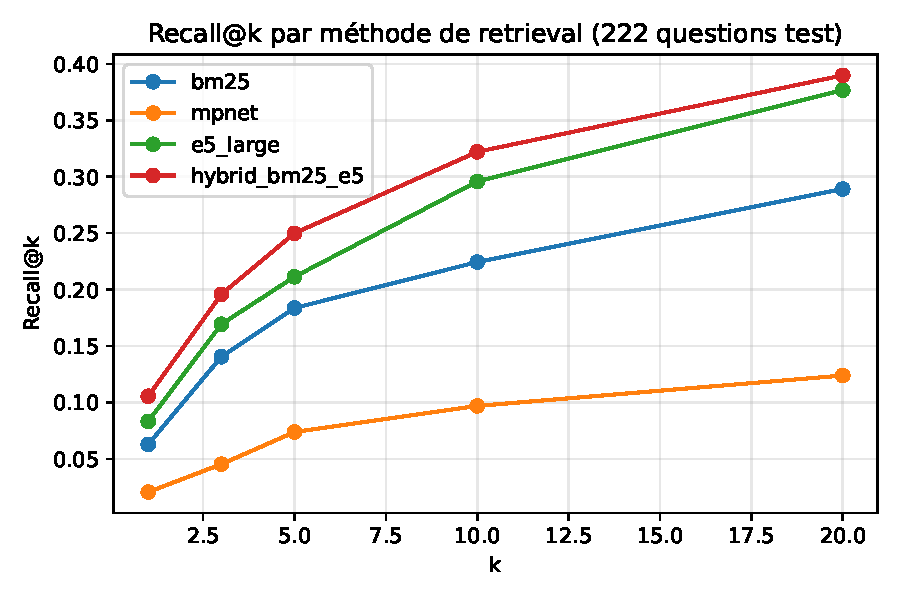
\includegraphics[width=\linewidth]{latex_assets/figs/recall_at_k_comparison.pdf}
\caption{Recall@$k$ as a function of $k$ for the four retrieval methods compared, full 222 question test split.}
\label{fig:recallk}
\end{figure}

\section{Fine-Tuning Extended to Several Configurations}
\label{sec:finetune}

The previous single fine-tuning run left open how sensitive the result was to the random seed, the amount of training data, the rank of the adapter and which parts of the network it touches, none of which a single run can answer. This phase therefore replaces that single run with a small family of runs that vary exactly one factor at a time wherever possible.

Fine-tuning still relies on a low rank adapter added to a frozen, quantized copy of Mistral. Instead of updating the full weight matrix $W_0$ of a linear layer, a low rank update is learned and added to it, $W' = W_0 + BA$, where $B$ has shape $d \times r$, $A$ has shape $r \times k$ and the rank $r$ is chosen far smaller than either dimension, so that only $B$ and $A$ are trained while $W_0$ never changes. The base model itself is kept in 4 bit precision throughout training, which is what keeps the whole procedure feasible on a single consumer grade GPU.

\begin{figure*}[t]
\centering
\resizebox{\textwidth}{!}{%
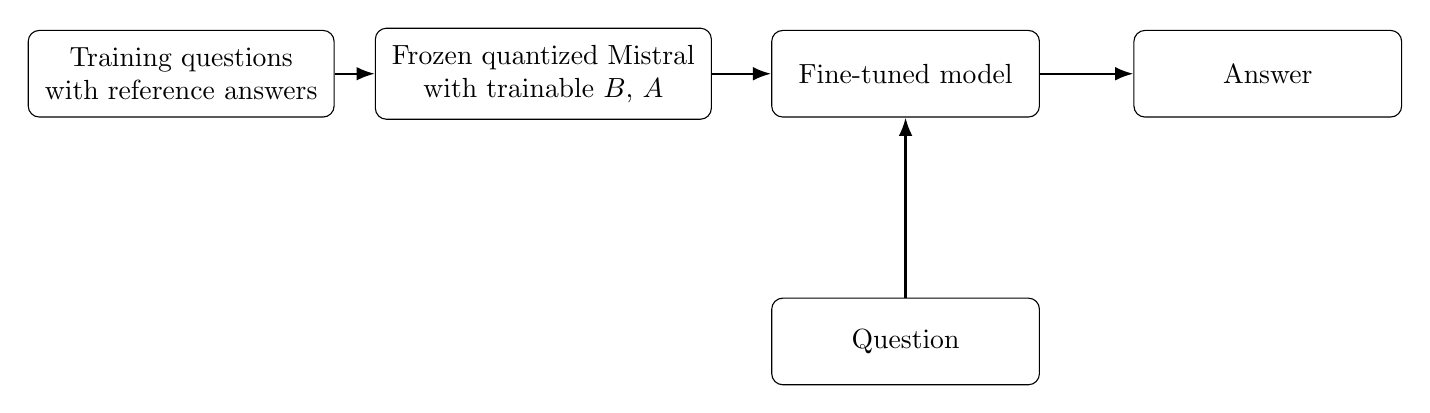
\begin{tikzpicture}[
  box/.style={draw, rounded corners, minimum height=1.1cm, minimum width=3.4cm, align=center, font=\normalsize, inner sep=6pt},
  arr/.style={-{Latex}, thick}
]
\node[box] (pairs)  at (0,1.7)   {Training questions\\with reference answers};
\node[box] (lora)   at (4.6,1.7) {Frozen quantized Mistral\\with trainable $B$, $A$};
\node[box] (tuned)  at (9.2,1.7) {Fine-tuned model};
\node[box] (question) at (9.2,-1.7) {Question};
\node[box] (answer) at (13.8,1.7) {Answer};
\draw[arr] (pairs) -- (lora);
\draw[arr] (lora) -- (tuned);
\draw[arr] (question) -- (tuned);
\draw[arr] (tuned) -- (answer);
\end{tikzpicture}}
\caption{Fine-tuning pipeline. Training questions and their reference answers update only the low rank matrices $B$ and $A$ of the adapter, while the quantized base weights $W_0$ stay frozen throughout. At inference time the resulting fine-tuned model answers a question directly, with no retrieval step involved.}
\label{fig:ftdiagram}
\end{figure*}

The adapter rank was raised from 16 to 32 this phase, on 580 training questions rather than 380, since a larger training set had become available and the additional adapter capacity was found to help rather than to overfit once a validation split existed to check for it. That validation split, 100 questions held out with a fixed seed independent of every other random choice in the pipeline, is itself a direct answer to a limitation of the previous phase, where only the training loss was tracked and there was no way to tell a model that generalizes from one that memorizes its 380 examples.

\begin{table}[H]
\centering
\small
\begin{tabular}{lcccc}
\toprule
\textbf{Variant} & \textbf{$n$} & \textbf{$r$} & \textbf{Train loss} & \textbf{Val loss} \\
\midrule
main (seed 42) & 580 & 32 & 0.834 & 0.679 \\
seed 123 & 580 & 32 & 0.844 & 0.689 \\
seed 2026 & 580 & 32 & 0.850 & 0.689 \\
$n=190$ & 190 & 32 & 1.122 & 1.098 \\
$n=380$ & 380 & 32 & 0.966 & 0.860 \\
$n=786$ & 786 & 32 & 0.736 & 0.561 \\
rank 8 & 580 & 8 & 0.850 & 0.710 \\
attention and MLP & 580 & 32 & 0.527 & 0.416 \\
plus synthetic data & 2580 & 32 & 0.940 & 0.516 \\
\bottomrule
\end{tabular}
\caption{Fine-tuning variants. All use Mistral-7B-Instruct in 4 bit precision, three epochs, and the same 100 question validation split.}
\label{tab:finetune}
\end{table}

Repeating the main configuration over three random seeds gives a final training loss of $0.843 \pm 0.006$, showing the training objective itself is stable, while the quality of the generated answers downstream turns out to vary considerably more across the same three seeds, a distinction the training loss alone cannot reveal and that only becomes visible once full generation and evaluation is repeated for every seed, as done in Section~\ref{sec:fourconfig}. Extending the adapter to the feed forward layers in addition to attention, or adding synthetic paraphrase questions to the training set, both lower the validation loss substantially, to 0.416 and 0.516 respectively, at the cost of a noticeably larger gap between training and validation loss, which is the signature of a model fitting its training distribution more tightly without a guarantee that the extra fit transfers to genuinely new questions.

\begin{figure}[H]
\centering

\includegraphics[width=\linewidth]{latex_assets/figs/learning_curve.pdf}
\caption{Final training and validation loss as a function of the number of training questions, rank 32 attention only adapter. The point near 330 examples corresponds to a specialist adapter trained on a narrower legal domain rather than the general training set, discussed in Section~\ref{sec:specialist}, and sits off the general trend for that reason.}
\label{fig:learningcurve}
\end{figure}

The earlier report's headline fine-tuning numbers, obtained on a 50 question subsample, were a ROUGE-L of 0.161 and a BERTScore F1 of 0.704 for the same rank 32, 580 example configuration. Under the present protocol, evaluated on the full 222 question test split with the confidence interval reported in Table~\ref{tab:generation}, the identical configuration gives a ROUGE-L of 0.147 with a 95 percent interval of 0.136 to 0.160. The earlier point estimate sits just outside the upper edge of that interval. Rather than trying to reconcile the two numbers, this is read as a demonstration of exactly why a 50 question subsample and a 222 question test split can disagree by an amount that matters, purely from sampling variance, and why every number reported from this point onward carries an interval alongside it.

\section{Four Configurations, Repeated and Bounded}
\label{sec:fourconfig}

A single point estimate cannot on its own say whether an observed difference between two systems reflects a genuine effect or the particular sample of 222 questions used to measure it. This phase therefore evaluates every configuration together with a bootstrap confidence interval and tests every pairwise comparison for significance rather than reading the ranking of the raw means directly.

Four configurations are compared under an identical prompt template, so that differences in the numbers reflect the technique rather than an accidental difference in how the model was asked. The zero shot configuration uses the base model with no added context. The retrieval configuration adds the top five articles found by the hybrid retriever. The fine-tuned configuration replaces the base model with the adapter from Section~\ref{sec:finetune} and adds no context. The fourth configuration combines both, the fine-tuned model with retrieved context, which the previous report's three way comparison did not include and which is the only way to see whether the two techniques stack.

The bootstrap confidence interval is obtained by resampling the 222 questions with replacement one thousand times, recomputing the mean ROUGE-L on each resample, and reading the 2.5th and 97.5th percentile of the resulting distribution of means as the interval bounds. This makes no assumption about the shape of the underlying distribution of scores, which matters here since per question ROUGE-L is far from a symmetric bell shaped quantity.

\begin{table}[H]
\centering
\small
\begin{tabular}{lcc}
\toprule
\textbf{Config} & \textbf{ROUGE-L} & \textbf{95\% interval} \\
\midrule
Zero-shot & 0.110 & 0.104 to 0.116 \\
RAG & 0.140 & 0.129 to 0.151 \\
Fine-tune & 0.147 & 0.136 to 0.160 \\
Fine-tune + RAG & 0.179 & 0.157 to 0.202 \\
\bottomrule
\end{tabular}
\caption{ROUGE-L with bootstrap 95 percent intervals, full 222 question test split, main seed.}
\label{tab:generation}
\end{table}

\begin{figure}[H]
\centering

\includegraphics[width=\linewidth]{latex_assets/figs/config_comparison_ci.pdf}
\caption{ROUGE-L with bootstrap confidence intervals for the four configurations.}
\label{fig:configci}
\end{figure}

Whether a difference between two configurations is genuine rather than noise is tested twice for every pair, once with a paired bootstrap test on the difference in means and once with the Wilcoxon signed rank test, which instead ranks the per question differences and sums the ranks of the positive and negative differences separately. The two tests rest on different assumptions, the Wilcoxon test in particular assumes the distribution of differences is symmetric around its median, so agreement between the two is a stronger form of evidence than either alone. Because six pairwise comparisons are drawn from the same four configurations, a Holm-Bonferroni correction is applied, which orders the six raw p values from smallest to largest and compares the $i$-th smallest to $\alpha / (6 - i + 1)$ rather than to a fixed threshold, which controls the chance of a false positive across the whole family of tests rather than for a single comparison taken in isolation.

\begin{table}[H]
\centering
\small
\begin{tabular}{lccc}
\toprule
\textbf{Comparison} & \textbf{$p$ boot} & \textbf{$p$ Wilc.} & \textbf{Sig.} \\
\midrule
Zero-shot vs RAG & $<$0.0001 & $<$0.0001 & yes \\
Zero-shot vs Fine-tune & $<$0.0001 & $<$0.0001 & yes \\
Zero-shot vs Combined & $<$0.0001 & $<$0.0001 & yes \\
RAG vs Fine-tune & 0.296 & 0.080 & no \\
RAG vs Combined & $<$0.0001 & 0.0002 & yes \\
Fine-tune vs Combined & 0.004 & 0.307 & mixed \\
\bottomrule
\end{tabular}
\caption{Paired significance tests, Holm-Bonferroni corrected across the six comparisons.}
\label{tab:sig}
\end{table}

Adding retrieval or fine-tuning individually both beat the zero shot baseline decisively and by a wide margin under both tests. Retrieval and fine-tuning taken alone are not distinguishable from each other, both tests agree on this, which on its own already says the two techniques are closer in overall lexical quality than the raw means in Table~\ref{tab:generation} might suggest. The comparison between fine-tuning alone and the combined configuration is the one pair where the two tests disagree, the bootstrap test calls it significant while Wilcoxon does not, which is treated here as a genuinely unresolved comparison rather than settled in favour of the test that happens to support the more attractive story.

\section{Looking Inside the Categories}
\label{sec:category}

An average taken across all 222 questions can hide very different behaviour in different areas of law, and the dataset happens to provide seven native legal categories that make this directly checkable rather than requiring a separate annotation effort.

\begin{figure}[H]
\centering

\includegraphics[width=\linewidth]{latex_assets/figs/heatmap_category.pdf}
\caption{ROUGE-L by configuration and legal category.}
\label{fig:heatmap}
\end{figure}

The gain from combining fine-tuning with retrieval is far from uniform across categories, it is largest for Logement and Argent and essentially absent for Travail, where the fine-tuned model alone already matches or beats the combined configuration. Two categories, Protection sociale with four questions and Travail with six, are explicitly flagged here as too small to support any claim about that category on its own, they are shown for completeness rather than treated as evidence.

\section{Where Does the Remaining Error Come From}
\label{sec:oracle}

Sections~\ref{sec:retrieval} and~\ref{sec:fourconfig} leave one question unanswered together, when retrieval based generation falls short of what seems achievable, is the fault with finding the right article or with using it once found. An experiment was designed specifically to separate the two, the true gold articles are placed directly into the prompt without going through the retriever at all, giving an oracle condition that removes retrieval error entirely while leaving every other part of the pipeline untouched.

\begin{table}[H]
\centering
\small
\begin{tabular}{lccc}
\toprule
\textbf{Condition} & \textbf{ROUGE-L} & \textbf{Exact match} & \textbf{Halluc.} \\
\midrule
Zero-shot & 0.110 & 0.005 & 0.144 \\
RAG (real retrieval) & 0.140 & 0.036 & 0.234 \\
Oracle context & 0.252 & 0.311 & 0.117 \\
\bottomrule
\end{tabular}
\caption{Oracle context ceiling, base (non fine-tuned) model throughout.}
\label{tab:oracle}
\end{table}

The gap in exact match citation rate between real retrieval and the oracle condition is 27.5 percentage points, against a gap of only half a point between real retrieval and no context at all. Almost the entire achievable improvement from retrieval is therefore gated by finding the right article rather than by the model's ability to use a correct one once given it. A second and less expected observation is that the hallucination rate is higher under real retrieval, 0.234, than with no context whatsoever, 0.144, and higher still than under the oracle condition, 0.117. Handing the model a plausible but wrong article appears to invite more confident fabrication than handing it nothing, which nuances any assumption that adding context can only ever help or at worst do no harm.

\section{Checking the Finding on a Second Model}

A pattern found on a single base model always leaves open whether it reflects something about legal question answering in general or something specific to Mistral. The same zero shot and retrieval protocol was therefore run unchanged on Qwen2.5-7B-Instruct, a comparably sized but architecturally distinct model, using the same 222 questions.

\begin{table}[H]
\centering
\small
\begin{tabular}{lccc}
\toprule
\textbf{Config (Qwen2.5-7B)} & \textbf{ROUGE-L} & \textbf{Exact match} & \textbf{Halluc.} \\
\midrule
Zero-shot & 0.105 & 0.000 & 0.180 \\
RAG & 0.131 & 0.027 & 0.360 \\
\bottomrule
\end{tabular}
\caption{Second base model, identical protocol.}
\label{tab:qwen}
\end{table}

The same qualitative pattern reproduces, retrieval improves lexical overlap and citation accuracy while roughly doubling the hallucination rate relative to zero shot. Finding this on an architecturally distinct model makes it considerably less plausible that the retrieval induced hallucination effect from Section~\ref{sec:oracle} is a quirk specific to Mistral.

\section{How Much Context Is Enough}

The production pipeline retrieves five articles for every question, a number chosen somewhat arbitrarily in the earlier phase. Since Section~\ref{sec:oracle} shows retrieval quality is the main lever available, it was worth checking directly whether more retrieved context is simply better.

\begin{table}[H]
\centering
\small
\begin{tabular}{lccc}
\toprule
\textbf{$k$} & \textbf{ROUGE-L} & \textbf{Exact match} & \textbf{Halluc.} \\
\midrule
1 & 0.135 & 0.02 & 0.14 \\
3 & 0.150 & 0.04 & 0.24 \\
10 & 0.136 & 0.02 & 0.20 \\
\bottomrule
\end{tabular}
\caption{Retrieval depth ablation, 50 question subsample.}
\label{tab:kablation}
\end{table}

Quality peaks at $k=3$ on every metric reported here and $k=10$ does not improve citation accuracy over $k=1$ despite carrying more than ten times as much context on average, which points to a dilution effect once the context grows large enough that the relevant article becomes harder for the model to weight correctly among the surrounding text. The production choice of $k=5$ sits close enough to this empirical optimum that it was left unchanged for the rest of this phase.

\section{Does the System Know What It Does Not Know}

None of the metrics above says anything about a question the system should refuse to answer altogether. A set of 50 questions was built specifically to test this, questions with no legal content at all, questions about a foreign legal system BSARD does not cover, and questions referencing an article that has since been withdrawn from the index.

\begin{table}[H]
\centering
\small
\begin{tabular}{lcc}
\toprule
\textbf{Config} & \textbf{Correct abstention} \\
\midrule
Zero-shot & 0.0\% \\
RAG & 2.0\% \\
\bottomrule
\end{tabular}
\caption{Correct abstention rate on 50 out of scope questions.}
\label{tab:abstention}
\end{table}

The system essentially never declines to answer, even for a question with no legal content whatsoever, it fabricates a plausible sounding legal answer complete with invented article numbers in nearly every case. This is the clearest negative finding of the whole phase and one that neither retrieval nor fine-tuning currently addresses.

\section{Two Different Notions of Quality}
\label{sec:judge}

Lexical overlap with a reference text and whether an answer actually addresses the question asked are not the same thing, and conflating them under a single score would hide which of the two is failing. Two separate measurements were introduced this phase for that reason, one entirely deterministic and one relying on an independent judge model, kept deliberately apart rather than merged into a single number\footnote{This separation, together with the specific choice of measuring citation grounding through named entity and number overlap rather than through a second LLM judgment, follows the methodological approach taken by Bouvard, Ciancone, Gourru and Schaeffer in their comparative evaluation of RAG and fine-tuning (APIA 2024), reimplemented here rather than reused directly.}.

The deterministic measure extracts named entities, numbers, email addresses and web addresses from both the generated answer and the reference text, calling this set of items the interest passages of a text, and reports what fraction of the interest passages in the generated answer also appear in the reference,

\begin{equation}
\text{fidelity} = \frac{|PI_{\text{response}} \cap PI_{\text{fragment}}|}{|PI_{\text{response}}|}.
\end{equation}

\begin{table}[H]
\centering
\small
\begin{tabular}{lc}
\toprule
\textbf{Config} & \textbf{Mean fidelity} \\
\midrule
Zero-shot & 0.054 \\
RAG & 0.295 \\
Fine-tune & 0.298 \\
Fine-tune + RAG & 0.324 \\
\bottomrule
\end{tabular}
\caption{Fidelity, entity and number overlap with the reference text.}
\label{tab:fidelity}
\end{table}

Relevance, whether the answer addresses what was actually asked independently of whether its content is correct, is instead scored by Phi-3.5-mini-instruct acting as an independent judge on a 50 question subsample. Because a single greedy judgment from a language model is a noisy point estimate, each answer is scored ten times at a temperature of 0.7 and the ten scores are averaged rather than trusting one sample.

\begin{table}[H]
\centering
\small
\begin{tabular}{lccc}
\toprule
\textbf{Config} & \textbf{Mean /5} & \textbf{\% scored 5} & \textbf{\% $\leq$3} \\
\midrule
Zero-shot & 5.000 & 100.0\% & 0.0\% \\
RAG & 4.850 & 90.2\% & 2.7\% \\
Fine-tune & 4.731 & 86.3\% & 3.3\% \\
Combined & 4.617 & 77.1\% & 4.6\% \\
\bottomrule
\end{tabular}
\caption{LLM judge relevance scores and score distribution.}
\label{tab:judge}
\end{table}

\begin{figure}[H]
\centering
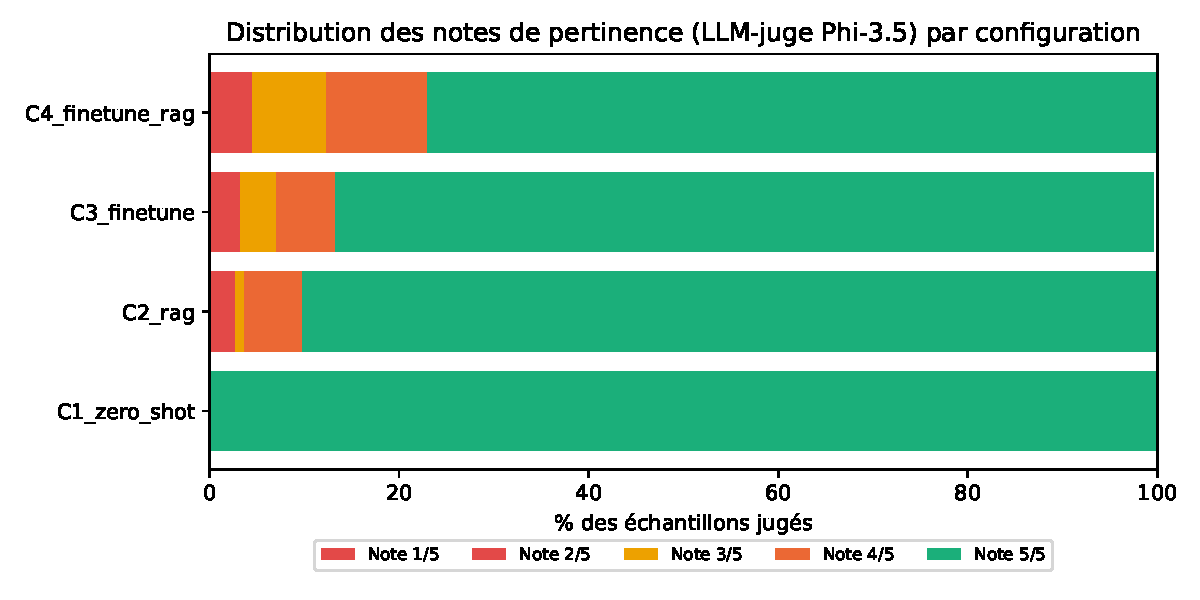
\includegraphics[width=\linewidth]{latex_assets/figs/llm_judge_pertinence_distribution.pdf}
\caption{Distribution of relevance scores by configuration, showing the growing tail of low scores hidden by the mean alone.}
\label{fig:judgedist}
\end{figure}

The mean relevance score alone stays high and nearly flat across configurations, yet the full distribution reveals a small but steadily growing share of clearly off topic answers moving from zero shot toward the combined configuration, from zero percent to close to five percent scored three or below. Read together with the qualitative observations in Section~\ref{sec:qualitative}, this indicates that adding retrieval or fine-tuning occasionally pulls the answer away from the specific question asked, a real but comparatively minor effect next to the citation grounding gap documented in Sections~\ref{sec:fourconfig} and~\ref{sec:oracle}.

\section{What Makes a Question Hard}

Two candidate explanations for why some questions are answered better than others were tested directly rather than assumed, the length of the question in words and the number of statutory articles genuinely required to answer it correctly, using the Spearman rank correlation between each candidate and the ROUGE-L obtained. Spearman correlation replaces raw values by their ranks before computing the ordinary correlation coefficient, which makes it sensitive to a monotonic relationship rather than specifically a linear one and less sensitive to a handful of extreme values.

\begin{table}[H]
\centering
\small
\begin{tabular}{lcc}
\toprule
\textbf{Config} & \textbf{$\rho$ length} & \textbf{$\rho$ n. articles} \\
\midrule
Zero-shot & $-0.107$ & $-0.452$\rlap{$^{*}$} \\
RAG & $-0.076$ & $-0.336$\rlap{$^{*}$} \\
Fine-tune & $-0.064$ & $-0.510$\rlap{$^{*}$} \\
Combined & $-0.152$\rlap{$^{*}$} & $-0.353$\rlap{$^{*}$} \\
\bottomrule
\end{tabular}
\caption{Spearman correlation with ROUGE-L. $^{*}$ significant at $p<0.05$.}
\label{tab:spearman}
\end{table}

Question length carries almost no relationship with answer quality, it is not even significant in three of the four configurations. The number of articles required to answer correctly, on the other hand, is a strong and highly significant negative correlate in every configuration, meaning length was the wrong proxy for difficulty all along and the real driver is how many separate rules must be combined into one answer.

\begin{figure}[H]
\centering
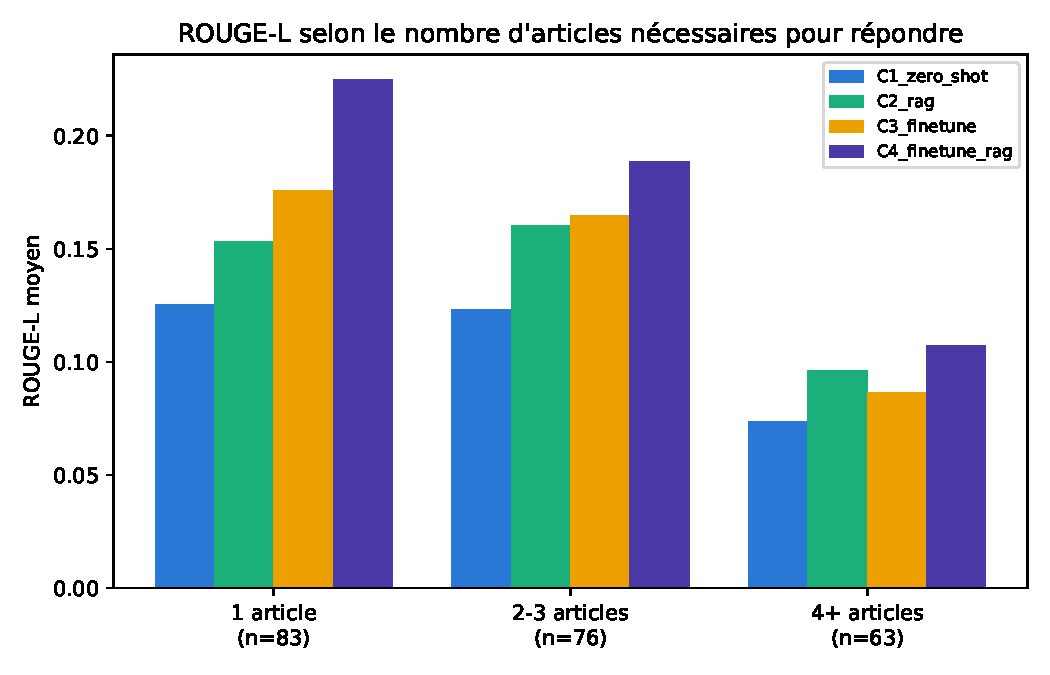
\includegraphics[width=\linewidth]{latex_assets/figs/difficulty_bucket_rouge.pdf}
\caption{ROUGE-L grouped by number of gold articles required, all four configurations.}
\label{fig:difficulty}
\end{figure}

Grouping questions by this count makes the effect concrete, quality stays broadly stable for one to three articles and then drops sharply once four or more must be combined, in every configuration without exception. Neither retrieval nor fine-tuning corrects this, combining several statutory provisions into a single coherent answer remains a limitation of the pipeline as it currently stands rather than something either technique happens to fix as a side effect.

\section{Can Reliability Be Predicted in Advance}

If certain kinds of questions are known in advance to be harder, as Section~\ref{sec:category} and the previous section both suggest, it becomes natural to ask whether an unreliable answer could be flagged before it is even shown to a user, using only information available before generation. A logistic regression and a random forest were trained with five fold cross validation to predict whether a given answer will achieve exact citation match, using question length, number of gold articles, category frequency in the training data, citation format and configuration as the only inputs.

\begin{table}[H]
\centering
\small
\begin{tabular}{lc}
\toprule
\textbf{Model} & \textbf{AUC} \\
\midrule
Logistic regression & 0.878 \\
Random forest & 0.838 \\
Majority class baseline & 0.500 \\
\bottomrule
\end{tabular}
\caption{Citation reliability classifier, area under the ROC curve.}
\label{tab:mlpred}
\end{table}

Both models separate reliable from unreliable answers far better than chance, keeping in mind that exact citation match is a rare positive outcome overall so the AUC should be read alongside that imbalance rather than in isolation. Question length, category frequency and the number of gold articles come out as the three strongest predictors, all three available before a single token is generated, which suggests a simple pre-flight check could plausibly flag low confidence questions for closer review in a deployed setting, a direction worth exploring further before the final report.

\section{A Domain Specialist Adapter}
\label{sec:specialist}

Looking inside categories in Section~\ref{sec:category} raises a natural next question, would an adapter trained only on one legal domain do better on that domain than a generalist adapter trained on everything at once. The Code Civil was chosen for this test since it covers a large share of the test questions, and a specialist adapter was trained on the 331 training questions that touch this code only, then compared against the generalist adapter on the same test questions split by whether they touch the Code Civil or not.

\begin{table}[H]
\centering
\small
\begin{tabular}{lcccc}
\toprule
& \multicolumn{2}{c}{ROUGE-L} & \multicolumn{2}{c}{Halluc.} \\
\textbf{Subset} & \textbf{Gen.} & \textbf{Spec.} & \textbf{Gen.} & \textbf{Spec.} \\
\midrule
In domain (FT) & 0.171 & 0.181 & 0.047 & 0.151 \\
Out domain (FT) & 0.132 & 0.123 & 0.052 & 0.022 \\
In domain (FT+RAG) & 0.215 & 0.151 & 0.151 & 0.081 \\
Out domain (FT+RAG) & 0.157 & 0.135 & 0.177 & 0.103 \\
\bottomrule
\end{tabular}
\caption{Specialist versus generalist adapter, Code Civil subset. Gen. is the 580 example generalist adapter, Spec. the 331 example specialist adapter.}
\label{tab:specialist}
\end{table}

The result is reported here as genuinely mixed rather than framed as a clean success. On its own domain, the specialist adapter alone is marginally better on ROUGE-L but hallucinates three times more than the generalist, and once combined with retrieval the specialist underperforms the generalist on ROUGE-L in both domains while hallucinating less in both. One confound has to be stated plainly, the specialist was trained on 331 examples against the generalist's 580, so a smaller training set is mixed together with narrower domain focus in this comparison, and Section~\ref{sec:finetune} already shows fewer examples alone lower quality. This experiment does not show that domain specialization fails, it shows that this particular version of the experiment cannot separate the two explanations, which is why a matched training set size is planned as a follow up rather than treating either reading of Table~\ref{tab:specialist} as final.

\section{Human Judgment Alongside the Metrics}

Every metric above is automatic, and an automatic metric can agree with itself while still disagreeing with what a human reader would actually prefer. Three annotators, the two authors of this report and a third annotator whose data collection is still in progress, independently and blindly compared the retrieval configuration against the fine-tuned configuration over 60 questions, with the side shown first randomized per question to avoid a positional bias.

Agreement between the two annotators with complete data is measured with Cohen's kappa, which corrects the raw agreement rate for the agreement expected by chance alone,

\begin{equation}
\kappa = \frac{p_o - p_e}{1 - p_e},
\end{equation}

with $p_o$ the observed proportion of questions on which the two annotators gave the same verdict and $p_e$ the proportion expected if each annotator answered independently at their own observed base rates.

\begin{table}[H]
\centering
\small
\begin{tabular}{lcccc}
\toprule
\textbf{Annotator} & \textbf{RAG} & \textbf{Fine-tune} & \textbf{Tie} & \textbf{Neither} \\
\midrule
Annotator 1 & 70.0\% & 10.0\% & 8.3\% & 11.7\% \\
Annotator 2 & 55.0\% & 8.3\% & 15.0\% & 21.7\% \\
\bottomrule
\end{tabular}
\caption{Blind pairwise preference between retrieval and fine-tuning, 60 shared questions.}
\label{tab:arena}
\end{table}

Cohen's kappa on the 60 shared questions comes out at 0.389, a fair to moderate level of agreement worth stating honestly rather than assuming two annotators following the same instructions will naturally agree closely, a limitation discussed further below. Despite that moderate agreement, both annotators independently and clearly prefer the retrieval configuration to the fine-tuned one, by a wide margin. This sits in real tension with the earlier automatic comparison on 50 questions, which had found the fine-tuned model ahead of retrieval on both ROUGE-L and BERTScore. Rather than treating this as a contradiction to explain away, it is read as the clearest demonstration in this whole phase of why a small sample lexical comparison and a blind human preference judgment on the same two systems can point in different directions, and why both are now measured side by side instead of relying on either alone.

\section{Qualitative Observations}
\label{sec:qualitative}

Reading through the annotated answers directly, alongside the arena comparisons above, surfaces four recurring patterns worth describing individually rather than folding into a single error rate.

The first is a reversal of legal roles, an obligation attributed to the wrong party, a tenant where the answer should say landlord, a legal cohabitant where it should say spouse. The dataset generates near duplicate question templates across adjacent categories that differ by exactly this kind of substitution while the governing article differs in a subtle way, applying directly in one case and only by analogy in the other, which is precisely the kind of confusable pair a retriever or a generator can conflate.

The second is invented statutory text. Given that hallucination remains at 11.7 percent even under the oracle context condition in Section~\ref{sec:oracle}, and that abstention is essentially absent as shown above, at least part of this tendency appears to be a property of the base model rather than purely an artefact of poor retrieval, a plausible sounding legal register produced regardless of whether there is any real grounding behind it.

The third is a complete drift away from the question asked, consistent with the growing tail of low relevance scores in Section~\ref{sec:judge}, usually triggered by a retrieved passage that is topically adjacent but does not actually answer what was asked, with no mechanism in the current pipeline able to recognize that mismatch.

The fourth is a decoding artefact rather than a modelling or data limitation, generation currently uses purely greedy decoding with no repetition penalty, a known and well documented cause of repetitive loops on smaller models producing long structured text, and correcting this is a concrete and low cost item for the next round of generation.

A further limitation raised by the annotators themselves deserves to be stated plainly rather than smoothed over, neither is a trained legal professional, and telling a subtly wrong legal claim apart from a correct one, applies directly against applies only by analogy being the clearest example, can exceed what a non specialist can confidently verify from the shortened reference context shown in the arena interface. This is one reason the moderate kappa reported above should not be read as carelessness on either annotator's part.

\section{Practical Difficulties Encountered}

As in the previous report, this section lists the technical obstacles actually met this phase, with their diagnosis and the fix applied, in the same spirit of a practical recommendation rather than a narrative account.

The BSARD article identifier field turned out not to be uniformly numeric, roughly a third of identifiers follow regional formats specific to Wallonia or Brussels, and a further small fraction carry a scraping artefact suffix glued directly onto the identifier. A generalized extraction pattern with an explicit coverage check was needed before any citation based metric could be trusted, since silently treating a fraction of gold citations as empty would have inflated the apparent hallucination rate without raising any error.

No held out validation split existed for fine-tuning prior to this phase, which made it impossible to tell a model that generalizes from one that memorizes on only a few hundred examples. A small, seed fixed validation split identical across every run was added specifically to close this gap, and is what makes the comparison across adapter rank and target modules in Section~\ref{sec:finetune} interpretable rather than anecdotal.

Independent jobs without a shared local package, a deliberate choice to keep each computation independently runnable, meant a fix applied to one script, most notably saving intermediate results after every step of a multi step job rather than only at the very end, did not propagate automatically to the others and had to be reapplied by hand across the family of scripts that share the same weakness.

Kaggle's free tier quota of two simultaneous GPU sessions was consumed silently more than once by a browser interactive session left open in addition to jobs launched through the API, and pushing a corrected version of a running job does not stop the earlier, still running version on its own, both keep occupying a slot until the earlier one is stopped by hand from the web interface.

\section{Next Steps}

Before the final report, three items remain open from this phase specifically. The retrieval Recall@k discrepancy described in Section~\ref{sec:retrieval} needs to be resolved or at least narrowed down through a chunking and metadata enrichment ablation. The third annotator's arena data collection and a formal double annotated error taxonomy, mentioned but not detailed in Section~\ref{sec:qualitative}, need to be completed. Generation should be rerun with a corrected decoding configuration including a repetition penalty, to separate how much of the fourth qualitative pattern above is a fixable artefact from how much reflects a genuine limitation of the current models and data.

\begin{thebibliography}{9}

\bibitem{hu2022lora}
E. J. Hu et al.
\textit{LoRA: Low-Rank Adaptation of Large Language Models.}
ICLR 2022. arXiv:2106.09685.

\bibitem{dettmers2023qlora}
T. Dettmers et al.
\textit{QLoRA: Efficient Finetuning of Quantized LLMs.}
NeurIPS 2023. arXiv:2305.14314.

\bibitem{lewis2020rag}
P. Lewis et al.
\textit{Retrieval-Augmented Generation for Knowledge-Intensive NLP Tasks.}
NeurIPS 2020. arXiv:2005.11401.

\bibitem{gao2023survey}
Y. Gao et al.
\textit{Retrieval-Augmented Generation for Large Language Models: A Survey.}
arXiv:2312.10997, 2023.

\bibitem{bouvard2024derby}
C. Bouvard, M. Ciancone, A. Gourru, M. Schaeffer.
\textit{Derby LLM: Evaluation comparative des approches RAG et fine-tuning.}
APIA 2024. hal-04638460.

\bibitem{louis2021bsard}
A. Louis, G. Spanakis.
\textit{A Statutory Article Retrieval Dataset in French.}
ACL 2021. arXiv:2108.11792.

\bibitem{zhang2020bertscore}
T. Zhang, V. Kishore, F. Wu, K. Q. Weinberger, Y. Artzi.
\textit{BERTScore: Evaluating Text Generation with BERT.}
ICLR 2020. arXiv:1904.09675.

\bibitem{chiang2024arena}
W.-L. Chiang et al.
\textit{Chatbot Arena: An Open Platform for Evaluating LLMs by Human Preference.}
arXiv:2403.04132, 2024.

\bibitem{ovadia2023finetune}
O. Ovadia, M. Brief, M. Mishaeli, O. Elisha.
\textit{Fine-Tuning or Retrieval? Comparing Knowledge Injection in LLMs.}
arXiv:2312.05934, 2023.

\bibitem{balaguer2024ragvsft}
A. Balaguer et al.
\textit{RAG vs Fine-tuning: Pipelines, Tradeoffs, and a Case Study on Agriculture.}
arXiv:2401.08406, 2024.

\end{thebibliography}

\end{document}
